\documentclass{article}
\usepackage{graphicx}

% For psedocode
\usepackage{amsmath}
\usepackage{algorithm}
\usepackage[noend]{algpseudocode}

\DeclareMathOperator*{\argmax}{arg\!\max}

\usepackage{hyperref}

\usepackage{enumitem}
\setlist[description]{leftmargin=\parindent,labelindent=\parindent}

\begin{document}

\title{Explorations in Tetris}
\author{Matt Brenman}

\maketitle

\begin{abstract}
This paper describes in detail my final project for the class {\em Advanced Topics in Machine Learning: Learning, Planning and Acting in Complex Environments}, including the architecture used to build a simulator for Tetris and the way to create additional agents to run against the system. It also describes a few types of algorithms that were tested against the system and their results and future directions for the project.
\end{abstract}

\clearpage

\setcounter{tocdepth}{2}
\tableofcontents

\clearpage

\section{Introduction}

\subsection{Why Tetris?}
I chose to explore Tetris because it is very difficult to play well, and I enjoy playing the game myself. Trivial representations of game state lead to an enormous state space, where a unique board representation leads to $2^{200}$ possible boards. Furthermore, maximizing cleared rows, maxmizing tetrises, minimizing the maximum height, or maximizing the number of pieces player are all NP-complete problems \cite{NPHard}. This makes it infeasible to come up with a perfect Tetris algorithm that fully solves the problem offline. 

The game, however, does have some nice properties. Each action has a deteministic component, which is the placement of the piece, and a non-deterministic component, which are the upcoming pieces. The fact that the board, action list, and piece list all have finite sizes allows us to consider the game as a massive but finite Markov Decision Process.

Since Tetris is an MDP, there are many different possible approaches to the problem. I chose to build a simulator that allows different agent programs to be swapped in and out so that I was not tied down to any algorithm. This also allows others to build and test their own agents without having to rebuild a simulator.

\subsection{Project Goals}
My main goal was to build a working, modular system that allowed agents to be built by only implementing a simple interface.

My secondary goal was to build an agent to play the system, and I had the rough metric of playing well. I did not have any specific goal of the number of lines cleared for this metric other than a lot.

\section{System Architecture}
Here is an outline of the different components of the system and their functionality, as well as the reasons for the design choices that I made along the way.

\subsection{The Game}
The game works similarly to the standard Tetris implementation, but it does not directly follow the official Tetris guidelines. The goals of the game, the size of the board, and the piece set all remain unchanged, but the interaction dynamics were adapted for faster learning.

\subsection{Actions}
The standard Tetris rules allow the agent to control the piece as it falls, moving it side to side as well as spinning it mid fall to produce T-spins. This implementation simplifies the action set to one action per piece, where an action consists of a rotation of the piece and a column to place it. The full action list allows pieces to be placed under other pieces if there is space, which is not possible in this implementation. I assume that an agent playing with the full action set would choose to hard drop a piece most of the time, excluding circumstances where it would be beneficial to place the current piece under another piece. Since the agent's actions are limtied in the implementation from the beginning, the optimal policy would vary since it would never expect to have those actions later and would hopefully avoid situations where they would be necessary.

The implementation of this action set is significantly simpler, since the board updates and player actions happen in serial. In the standard version, the piece falls one space before an action is even played if enough time passes, which forces the agents to respond based on time as well. In this implementation, however, the agent could take as much time as needed, so it is up to the agent designers to follow a reasonable time constraint.

The transition function between board states decreases (and simplifies) with this action set, since it is deterministically activated (instead of being affected by time) and since there are fewer transitions from any state. The allows agents to learn more quickly, since they have less to explore, and it also decreases development time since the board state will not spontaneously change during computation.

\begin{figure}[ht!]
  \centering
    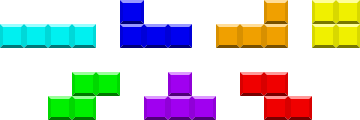
\includegraphics[scale=0.5]{standardtets.png}
  \caption{The Standard Tetromino Set \cite{standardtets}}
  \label{fig:standardtets}
\end{figure}

\begin{figure}[ht!]
  \centering
    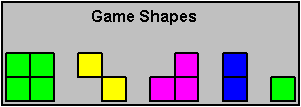
\includegraphics[scale=0.5]{smalltets.png}
  \caption{The Smaller Tetromino Set \cite{smalltets}}
  \label{fig:smalltets}
\end{figure}

\subsection{Pieces}
The tetrominoes used are the same set as the standard game, as shown in Figure~\ref{fig:standardtets}. Initially, I used the limited Tetromino set as shown in Figure~\ref{fig:smalltets}, but this task was figured out very quickly, since it is much easier to play. I then moved over to the standard set to give the agent a harder task. 

\subsection{Scoring}
This implementation uses a simplified version of the scoring mechanism. Instead of giving more points for larger line clears like in the standard version, this version rewards all line clears in a manner proportional to the number of lines cleared.

This, however, slightly changes the strategy. In the standard game, a Tetris, which is clearing four lines with one piece, earns more points than two clears that each clear two lines, and both earn more points than four clears of one line each. My implementation, however, does not discriminate between these, but the overall goal of clearing more lines stays the same.

\subsection{Using the Board}
The setup of the system allows agents to access the information of the gameboard while disallowing any modification of the official game board. This allows for trivial creation of simulators that directly model the current game. The simulators that are created for users do not allow users to see the pieces beyond the next piece, so there is no extra information gained from simulators above a human player.

The simulators, however, do allow agents to change parts of the current piece, which is useful if an agent wants to test with certain pieces (or with all of the pieces) without hoping that random simulations offer up those pieces. The official game, still, does not allow the agent to modify the game pieces.


\section{Agents}

\subsection{Random Agent}
\subsubsection{Motivation}
I created a random agent as a very simple demonstration of how to find which rotations and columns are available and how to return an action.
\subsubsection{Results}
The random agent does not play well, but this is to be expected from a random agent.

\subsection{Heuristic Agent}
\subsubsection{Motivation}
One reasonable way to evaulate an agent is to run it on a many games and average the number of lines cleared, but this is not the best metric for evaluating each action within a game. In order to evaluate a move, more information should be taken into account since not only do we want to clear lines, but we also want to make sure that we will have a nice board for future moves.

The heuristic agent takes into account many features and calculates the value of any move based on a linear combination of those features, which gives rise to the following equation:

\begin{equation} \label{heuristiclc}
Q(s,a) = f_{1}*w_{1} + f_{2}*w_{2} + \dots + f_{m}*w_{m}
\end{equation}

where \(\vec{f}\) is a vector of length \(m\) that represents the observed values of the chosen features, and \(\vec{w}\) is the weight vector that adjusts the influence of each of the features on the estimated value of the move. This allows us to choose an action with the following policy:

\begin{equation} \label{heuristiceq}
\pi_{Heuristic}(s) = \argmax_a \{ Q(s,a) \}
\end{equation}

\subsubsection{Implementation}
The usefulness of this algorithm depends entirely on the features chosen and their respective weights, since if the agent is observing irrelevant values or incorrectly weighting these features (avoiding line clears or rewarding height, for example) then the agent will perform terribly. For this reason, picking relevant features and appropriate weights is very important.

These were the features that my heuristic agent observes: 
\begin{description}
  \item[$\Delta$Lines Cleared] The number of lines that action \(a\) clears
  
  \item[$\Delta$Height] The change in maximum height  before and after action \(a\)
  
  \item[$\Delta$Holes] A hole is defined as a fully enclosed (either by a wall or by more pieces) section of empty spaces. This feature is the change in that number before and after action \(a\)
  
  \item[$\Delta$Blocked Spaces] A blocked space is any empty space that has a piece above it. This feature is the change in that number before and after action \(a\)
  
  \item[$\Delta$Aggregate Blocked Spaces] The aggregate blocked space is the number of pieces that are blocking an empty space. This feature is the change in that number before and after action \(a\)
  
  \item[Total Height] The sum of the height of every filled space
  
  \item[Lose Status] Whether or not the game is lost after performing action \(a\)
\end{description}

To find the weights that I ended up using for this agent, I used evolutionary programming, which is explained later in the paper, but hand-designed weights could be used too.

\subsubsection{Results}
The heuristic agent, when provided an appropriate set of features and weights, performs decently. It's downfall, however, is that is does not account for the knowledge of the next piece or do any simulations of what it think will happen next, which leads to a few more sophisticated approaches.

One of the most important changes to the project was the inclusion of the \emph{Total Height} feature. The first iteration only included \emph{$\Delta$Height}, which worked to keep height gain low between moves, but it meant that the agent did not act differently if it was close to losing. A more useful approach is to focus much more on getting the height down when the board is getting high, which is not possible to see only given \emph{$\Delta$Height}.

\subsection{Rollout Agent}
\subsubsection{Motivation}
Since the state space of Tetris is huge, forming an explicit policy for every state would take up a large chunk of memory and take very long to solve. Policy rollout allows us to simulate potential next states and approximate $Q(s,a)$ as the average discounted reward over the trajectories and picks the action as follows:

\begin{equation} \label{rollout}
\pi_{rollout}(s) = \argmax_a \{ Q(s,a) + \dfrac{1}{w}\displaystyle\sum^{w}\displaystyle\sum_{i=1}^{k} \gamma^{k}Q(s^{k}, \pi_{Heuristic}(s^{k}))\}
\end{equation}

where n is the number of trials, k is the length of the trajectories, and $s^{k}$ is the state after k moves have been taken (including the first action).

\subsubsection{Results}
Policy rollout performs well on Tetris when the agent uses many simulations and trajectories that are not that long. The length of each trajectory exponentially decreases the likelihood of encountering that trajectory, which is expressed here:

\begin{equation} \label{probtraj}
P(s^{k}|s,\pi^h) = \dfrac{1}{number\_of\_tetrominos^{k - 1}}
\end{equation}

where $s^{k}$ is the board state after k moves following heuristic policy $\pi^h$. Note that since, the first move is deterministic, $Pr(s'|s,\pi^h) = 1$. This makes it beneficial to keep the trajectory lengths low so that we explore more likely trajectories. On the other hand, if we make the trajectories too short, then the agent may unknowingly get itself into a bad situation.

The width of the rollout allows us to get a more accurate representation of the actual distribution of the next piece given to us during the transition function, so having a wide width is important. The length of each trajectory however, makes the sequence in the trajectory exponentionally less likely. The algorithm does very well, but the work needed to create all of the simulators and find the heuristic action makes the program take a while to run.


\subsection{Modified Rollout Agent}
\subsubsection{Motivation}
Standard policy rollout does not take into account information that is already known about the game. We know the next piece from the game, which makes the next state deterministic for any action $a$ taken in $s$. This allows us to simulate the first step before branching out, since we are guaranteed to get the same state. Standard policy rollout does not take this into account.

Furthurmore, the next piece (the only non-deterministic piece of the system) falls on a distribution that we can assume. The pieces seem to appear uniformly randomly (even though they are created with a bag system in the official rules), so we can greatly reduce the amount of work that we have to do to get a more accurate estimate.

Instead of increasing the width of the search, we can test all possible next pieces. This gives us an equal weighting of possible next steps, which appears to be what is happening in the game, but limits the computation time significantly.

\subsubsection{Results}
This agent takes significantly shorter time to make reasonable decisions. Even without the simulated possible pieces, the agent performs very well, clearing thousands of lines easily.

The speed of the computation of the heuristic function affects this agent's speed the most, and memoizing choices would greatly help this bottleneck. The problem could also be relaxed for this component, which would help as well.

\section{Improving the Agents}
Since the heuristic function plays such an important role in the agent's performance, I wanted to automate a process to find decent weights for the heuristic function. I chose a genetic algorithm, described below, that chose the weights used \cite{geneticideas}.

\subsection{Genetically Programming the Heuristic Function}
The genetic programming ideas that I used constisted of the following repeated steps:

\begin{description}
  \item[Evaluate] Over a certain number of trials, rank the agents by their average number of lines cleared
  \item[Replace the Weaklings] The worst half of the agents are replace by either mutation or cross-over.
\end{description}

For mutation, one of the surviving agents is chosen and each parameter is modified up to a certain amount (on the order of 1\%). This essentially performs hill-climbing over enough trials.

For cross-over, two surviving agents are chosen and the new agent is created by randomly choosing each weight from one of the two parents. This allows us to (hopefully) escape finding local maxima.

I also introduced random spawns to further decrease the likelihood of local minima, which acted like a lot of random restarts.

\subsubsection{Results}
The genetic programming algorithm provided weights that performed better than my hand chosen weights after a very short period of time. After improving the methods used here, I think that it could become a very strong method of choosing weights, especially when there are many features or the interplay between the features is not obvious.

\section{Future Work}

\subsection{Interface}
I would eventually like to make a GUI for this program that allows users to easily control the heuristic weights and test different weights without modifying any code. I would also like to allow for dynamic heuristics in the heuristic agent that are chosen at run-time by the user.

\subsection{Heuristic Work}
Since the heuristics and weights that are used are very important, I would like to spend more time optimizing this section.
\subsubsection{Feature Selection}
One idea that I have is to find a way to find the most salient features given a large list of features. Hand choosing the features allows for biases that I could introduce, so I'd like to avoid that if possible.
\subsubsection{Evolutionary Algorithm}
I would like to spend more time running the evolutionary algorithm, as well as optimizing how well it finds weights. I think that instead of taking the top performing of each generation, it could be useful to choose based on generational diversity as well as confidence of the score. Since we could store all of the scores that went into the average, we could calculate the variance of the average and use that as a measure of confidence in the score. I would much rather keep, for example, an agent with a score of 100 with 80\% confidence compared to an agent of 105 with a 40\% confidence. Many of these values (diversity criterion, mutation rate, random restart rate, etc) could start near 1 but anneal over time to ensure convergence of the algorithm.

\subsection{Different Tetromino Sets}

\subsubsection{Small Tetromino Set}
Allowing a smaller tetromino set (2x2 pieces) would allow more complicated algorithms to have an ``easy mode'' to use for testing.

\subsubsection{Tetracube Set}
I would like to expand the game to include tetracubes, which are 3-D versions of the standard tetrominoes. This would be a much more difficult game and may allow for some interesting new algorithmic design.

\subsection{Different gameplay}
Instead of only allowing the hard drop action, it would be nice to simulate the game exactly as it is played by humans. This would cause some problems, but with a little work, they could likely be resolved.

\section{Conclusion}
While my algorithm should be able to be expanded to play much better, I am very happy with how the project turned out. The simulator allows different agents to easy be used, and the agent system also allows agents to be created (even ones that use extensive simulation of dream games) easily. The maximum number of lines that I have seen the agents clear is over 36,000, which I am excited to try and beat.

\clearpage

\section{Using the Program}
\subsection{Compile}
Run $sh$ $compile$ from inside the directory.
\subsection{Running the Game}
Use $./play$ to run the game.
\subsection{Running the Training Algorithm}
Use $./train$ to run the genetic training algorithm.
\subsection{Incorporating Your Own Agent}
After writing your agent, include it in the $Game.cpp$ file and change line 24 of that file to create an instance of your agent. Add your file name to the compile scripts, then compile and run the program.
\clearpage

\begin{thebibliography}{1}

\bibitem{NPHard} Breukelaar, R., Demaine, E. D., Hohenberger, S., Hoogeboom, H. J., Kosters, W. A., and Liben-Nowell, D. (2004). Tetris is hard, even to approximate. International Journal of Computational Geometry and Applications, Vol. 14, pp. 41–68. Special Issue: Selected Papers from the Ninth International Computing and Combinatorics Conference (COCOON 2003), Big Sky, MT, USA, July 2003.

\bibitem{smalltets} Bdolah, Yael, and Dror Livnat. ``Reinforcement Learning Playing Tetris.'' Reinforcement Learning Final Project. N.p., 2000. Web. \url{<http://www.math.tau.ac.il/~mansour/rl-course/student_proj/livnat/tetris.html>.}

\bibitem{geneticideas} ``Coding a Tetris AI Using a Genetic Algorithm.'' Luckys Notes. N.p., 27 May 2011. Web. \url{<http://luckytoilet.wordpress.com/2011/05/27/coding-a-tetris-ai-using-a-genetic-algorithm/>.}

\bibitem{standardtets} McGarity. ``Watch Us Grow In...Ms.McGarity's Garden!'' : 1, 2, 3, 4...Tetrominoes Galore! N.p., n.d. Web. \url{<http://mcgaritysgarden.blogspot.com/2009/11/1-2-3-4tetrominoes-galore.html>.}

\end{thebibliography}

\end{document}